\documentclass[11pt,a4paper]{ivoa}
\input tthdefs
\input gitmeta
\usepackage[textsize=small,textwidth=3.8cm,backgroundcolor=yellow]{todonotes}

\title{IVOA Interoperable Authentication Management}

% see ivoatexDoc for what group names to use here; use \ivoagroup[IG] for
% interest groups.
\ivoagroup{Distributed Services and Protocols}

\author{Mark Taylor}
\author{Sara Bertocco}
\author{Patrick Dowler}
\author{Brian Major}

\editor{Mark Taylor}

% \previousversion[????URL????]{????Concise Document Label????}
\previousversion{This is the first public release}

\newcommand{\rfc}[1]{RFC\,#1}
\newcommand{\header}[1]{{\tt #1}}

\begin{document}

\begin{abstract}
IVOA's Interoperable Authentication Management explains how
VO services can manage the authentication process for
interoperability with clients, especially non-browser clients.
Particularly, this document
describes how services advertise their
support of specific authentication schemes and how
clients can discover and use this information to access protected
resources.
\end{abstract}


\section*{Acknowledgments}


\section*{Conformance-related definitions}

The words ``MUST'', ``SHALL'', ``SHOULD'', ``MAY'', ``RECOMMENDED'', and
``OPTIONAL'' (in upper or lower case) used in this document are to be
interpreted as described in IETF standard RFC2119 \citep{std:RFC2119}.

The \emph{Virtual Observatory (VO)} is a
general term for a collection of federated resources that can be used
to conduct astronomical research, education, and outreach.
The \href{https://www.ivoa.net}{International
Virtual Observatory Alliance (IVOA)} is a global
collaboration of separately funded projects to develop standards and
infrastructure that enable VO applications.


\section{Introduction}\label{sec:intro}

Historically many services in the VO have operated primarily or
entirely in anonymous mode.
However authentication and associated authorization
are becoming increasingly necessary in the VO,
for instance to manage data rights and as an operational necessity for
auditing and limiting service usage in the era of science platforms.
% Some way to manage authentication for VO services is therefore necessary
% but not covered in all contexts by existing industry-standard machinery.

Where the client is browser-based
a service can often integrate information about the authentication
methods required with the web page or web application through which
it is accessed.
\todo{is this true?  I don't understand browser-based authentication
      or what makes it work all that well}

But a desktop VO client such as Aladin, TOPCAT or Python
typically interacts with VO services differently, in one of two
ways:
\begin{enumerate}
\item Searches the registry for a service, then makes VO-compliant
      requests to that service (e.g.\ TAP)
\item Is presented with a URL, then retrieves the data from that URL
      (e.g.\ DataLink)
\end{enumerate}
In the first, TAP-like, case additional information is available to the
client in the form of the Registry record for the service in question,
as defined by VOResource \citep{2008ivoa.spec.0222P}
and its service-specific extensions.
This could in principle contain metadata describing the authentication
method along with any required ancillary information such as
login endpoints.
Even if only the TAP service URL is available
(for instance because the user has typed it in rather than acquired it
from a Registry search) the VOSI Capabilities endpoint can be reliably
located ({\tt /capabilities} is a sibling of {\tt /sync} in TAP),
so that relevant VOResource information could be retrieved from the VOSI
Capabilities document supplied by the service.

However in the second, DataLink-like, case
there is no information about where to find a corresponding
registry record or VOSI document,
or even a guarantee or likelihood that such a record exists.
The URL in question may not even have come from a DataLink query,
it could simply be a pointer to a protected resource like a
FITS file or VOTable in a secured filestore.
Such a URL may have been acquired from a VO query in the application
wishing to dereference it, in which case some authentication context
may be available,
but it may equally be read from a VOTable transmitted by SAMP
or saved in an earlier session, or obtained from an unrelated application;
in other words the application requiring the resource at a URL may
have no information about the VO service which produced that URL.
Then the only opportunity to acquire information about how to authenticate
is by examining the URL itself, or by HTTP communications with that URL.

An authentication method like HTTP Basic (\rfc{7617})
can be used in this scenario,
since all negotiation involving user credentials and permits ---
request and supply of username and password ---
is done directly
over the HTTP connection from which the resource is requested.
More modern/secure/flexible authentication methods however tend to
rely on additional interaction with other, unspecified, endpoints
prior to the request itself.  For instance OAuth2 requires presentation
of a Bearer Token to retrieve protected resources from a given URL,
but there is no way given only that URL to determine where or how
to acquire this token;
in a typical OAuth2 usage scenario such information is known up front
by the components making the request.

No industry standard mechanism appears to exist to solve the
problem of how a client can authenticate without such up-front
information.
This document therefore proposes some VO-standard mechanisms
by which a service can advertise to clients all the information
required to authenticate,
in particular how to exchange user credentials for an authentication permit,
given only the URL for a suitably compliant protected resource.

To address this, this document defines (Section~\ref{sec:authschemes})
some VO-specific authentication schemes
for use in \header{WWW-Authenticate} challenges.
It also describes (Section~\ref{sec:cr-use}) how to discover the
authentication requirements for VO services, and
some arrangements for working with optional authentication.

The intent of this document is not to define new authentication
mechanisms parallel to pre-existing standards, but to provide
missing components that facilitate use of such existing standards
from certain VO contexts, especially by non-browser clients.
Authenticated services in the VO are not expected to change their
authentication frameworks to any ``VO-sanctioned'' technology,
but by implementing the proposals here they can become usable
in a broader range of scenarios.
VO services however are not required to use any of the  
mechanisms proposed in this document; if they can establish the
client interoperability they require using other mechanisms
they are free to do so.

Given that, as explained above,
the VOResource record can only be discovered in some (TAP-like)
and not other (DataLink-like) authentication scenarios,
it is no longer recommended to base discovery of authentication methods
on the {\tt securityMethod} element
defined by VOResource, as described by SSO 2.0.
Instead, the proposal here is recommended for both TAP-like and DataLink-like
scenarios.

\subsection{Role within the VO Architecture}

\begin{figure}
\centering

% As of ivoatex 1.2, the architecture diagram is generated by ivoatex in
% SVG; copy ivoatex/archdiag-full.xml to role_diagram.xml and throw out
% all lines not relevant to your standard.
% Notes don't generally need this.  If you don't copy role_diagram.xml,
% you must remove role_diagram.pdf from SOURCES in the Makefile.

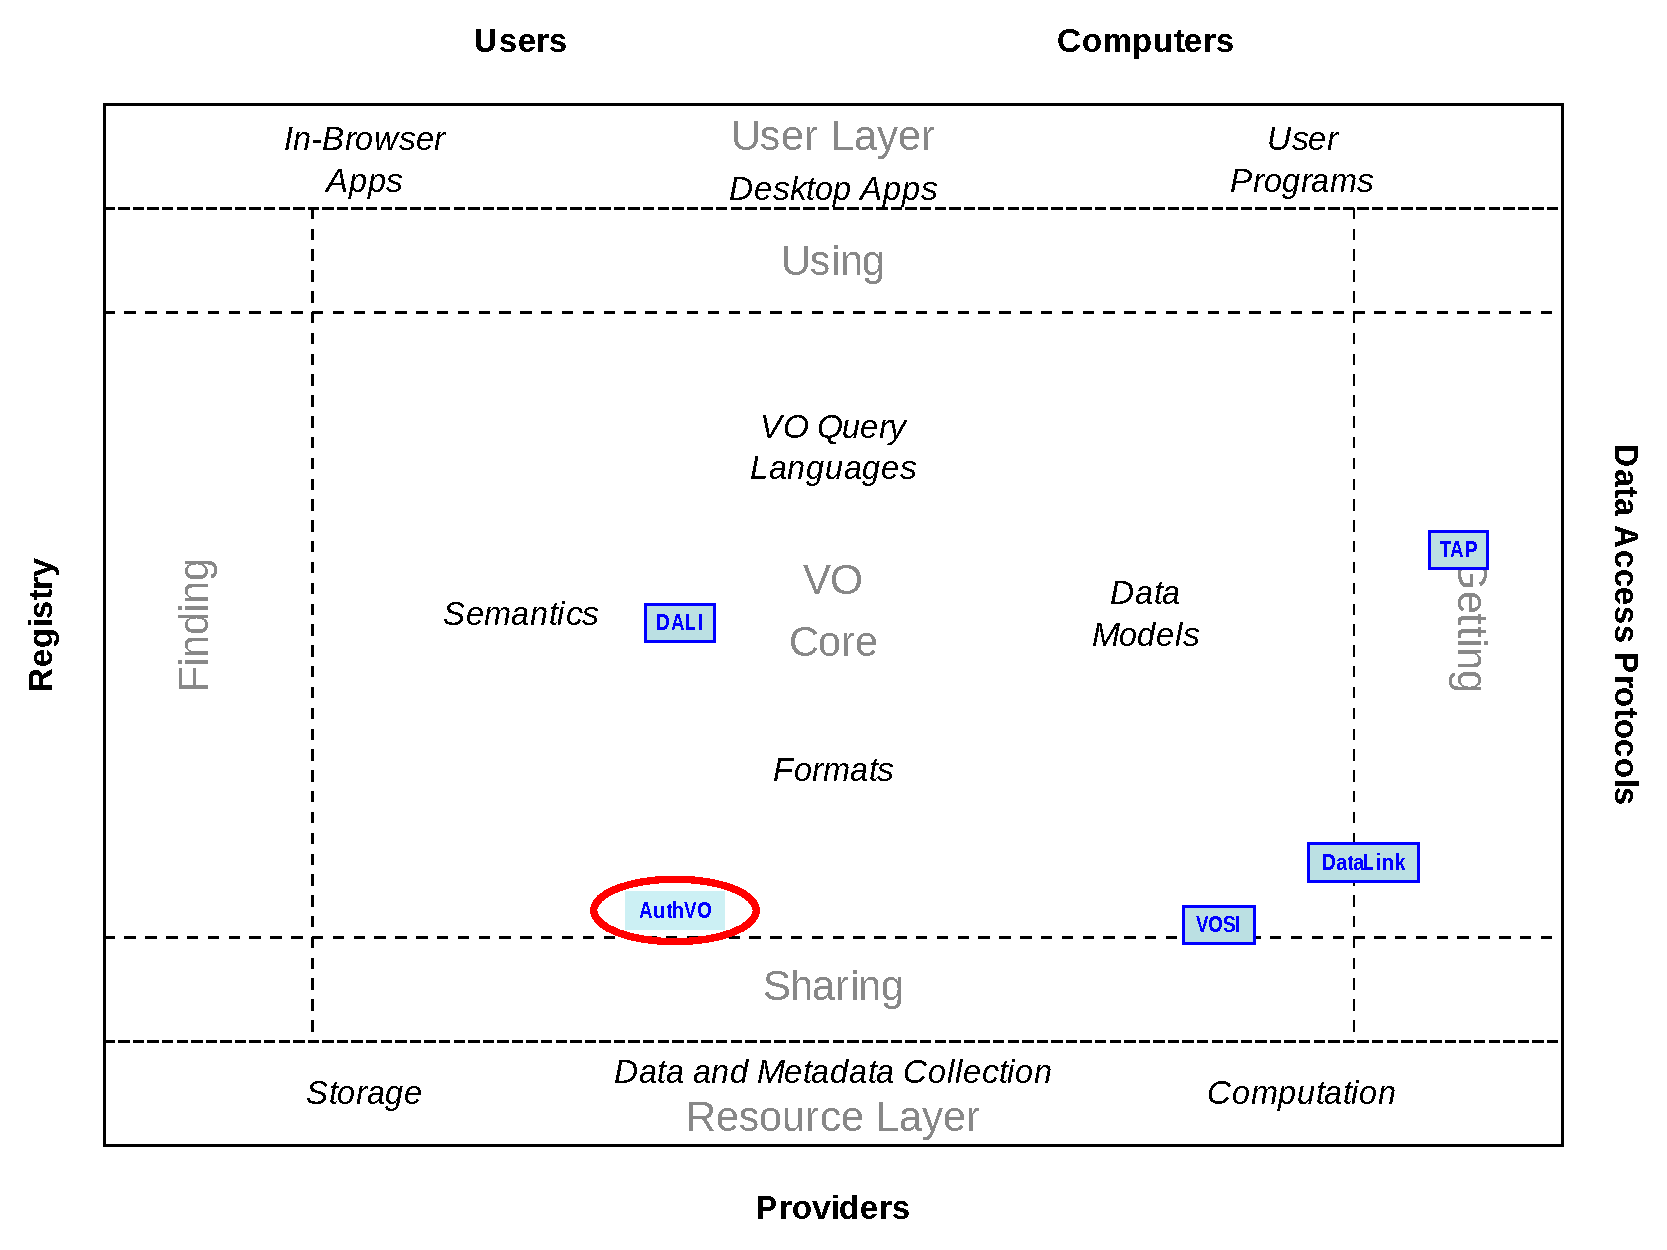
\includegraphics[width=0.9\textwidth]{role_diagram.pdf}
\caption{Architecture diagram for this document}
\label{fig:archdiag}
\end{figure}

Fig.~\ref{fig:archdiag} shows the role this document plays within the
IVOA architecture \citep{2021ivoa.spec.1101D}.

IVOA-IAM provides a way to advertise authentication methods
associated with existing VO services.
For services like TAP \citep{2019ivoa.spec.0927D}
that comply with VOSI \citep{2017ivoa.spec.0524G} to
offer service description documents at locations
defined by DALI \citep{2017ivoa.spec.0517D},
clients can discover these methods
using an up-front query to the VOSI capabilities endpoint.
For non-VOSI services such as DataLink \citep{2015ivoa.spec.0617D}
such discovery is done reactively.


\subsection{Terminology}

The following terms are used with specific meanings in this document:

\todo{Are these OK? Do they align with established usage?
      Are there better choices?}
\begin{description}
\item[protected]
      A service or resource that can only be accessed by authenticated users
\item[permit]
      Information that a client can supply with an HTTP request to
      prove its authenticated identity;
      may for instance be a token, cookie or certificate
\item[credentials]
      Secret information known to a user, such as a username and password,
      that can be used to acquire a {\em permit}
\item[authentication domain]
      A set of HTTP endpoints sharing the same authentication arrangements;
      the same {\em permit\/} is applicable to all members of the same domain
      and should not be presented to endpoints outside that domain
\item[challenge]
      A structured invitation to authenticate using
      a particular {\em permit\/} type,
      presented within a \header{WWW-Authenticate} header
\item[authentication scheme]
      A particular type of {\em challenge\/} with its own rules and syntax
\end{description}
The terms {\em challenge\/} and {\em authentication scheme} are
defined by \rfc{9110}
and explained further in Section~\ref{sec:challenge-response}.


\section{Challenge and Response}

The standard way to negotiate authentication over HTTP is using 
authentication challenges supplied in HTTP responses.

\subsection{Challenge/Response Framework}
\label{sec:challenge-response}

The basics of authentication over HTTP can be found in
section 11 of \rfc{9110} \citep{std:RFC9110};
that document obsoletes \rfc{7235} \citep{std:RFC7235}
which presented an earlier version of this protocol.
More detail can be found in those documents, but for convenience
the basics are outlined here:
% 401, 403, WWW-Authenticate, maybe Authorization.
\begin{itemize}
  \item An HTTP response may include one or more 
        \header{WWW-Authenticate} headers
        to indicate that authentication is possible.
        The content of these headers is one or more {\em challenges},
        each describing how the client can authenticate according
        to a named {\em authentication scheme}.
  \item A 401 (Unauthorized) response MUST include at least one such challenge
  \item Other (e.g. 200 OK, 403 Forbidden) responses
        MAY include such challenges
  \item The client may use the challenge information to decide how
        to authenticate itself to the server in subsequent requests.
        This can be done by supplying the \header{Authorization} header
        with scheme-specific content.
        In case of multiple challenges, the client is free to choose one.
  \item The form of a challenge is:\\
        \verb|   <auth-scheme-name> [<scheme-specific-parameters>]|
  \item The form of the \header{WWW-Authenticate} header is:\\
        \verb|   WWW-Authenticate: <challenge> [<challenge> ...]|
\end{itemize}

\todo{
   Do we need to worry about 407 and proxy-authenticate?
   I don't {\em think\/} so.
}

The details of a number of these authentication schemes
(\verb|<auth-scheme-name>| strings and their
associated parameters and semantics)
are defined in IETF documents, for instance
``{\tt basic}'' (\rfc{7617} \citet{std:RFC7617})
``{\tt digest}'' (\rfc{7616} \citet{std:RFC7616})
and
``{\tt bearer}'' (\rfc{6750} \citet{std:RFC6750}).
\rfc{9110} section 11.1 says
``New and existing authentication schemes are
  specified independently and ought to be registered''
  (\href{https://www.iana.org/assignments/http-authschemes}{with IANA}),
but it does not say that they MUST be so registered.



\subsection{Authentication Schemes in the VO}

Where one of the standard authentication schemes is
suitable for use by a particular VO service and its clients,
it should be used.
For instance Basic or Digest authentication provide all required
information about the authentication procedure within the headers,
since the client simply supplies
(somewhat obscured) username and password
to the target service in subsequent requests.
If these schemes are used it is highly recommended
to require a TLS connection (HTTPS not HTTP) to avoid interception of
the credentials.

Services using OAuth2 generally make use of the Bearer scheme.
In this case the challenged client supplies a {\em bearer token}
in subsequent requests,
but the challenge provides no information about how to acquire
such a token which means it is not suitable for clients lacking
prior knowledge about the target service, as described in
Section~\ref{sec:intro}.

Other methods of authentication over HTTP also exist
and are used by VO services,
for instance use of cookies and of X.509 certificates.
In standard usage these do not use \header{WWW-Authenticate} challenges,
and again prior knowledge about the service
(how to acquire a suitable cookie or certificate)
is required by the client to use them.

This document defines in \ref{sec:voschemes}
some VO-specific authentication schemes
that solve these problems by supplying the missing information to
clients in scheme-specific challenge parameters.

\section{Authentication Schemes}\label{sec:authschemes}

The authentication schemes defined in this section
generally define:
\begin{enumerate}
  \item How clients are to present a permit in future requests
        to a service --- this is defined by the identity of the scheme
  \item How they are to acquire such a permit ---
        this is communicated by the scheme-specific parameters
\end{enumerate}
Acquiring a permit (such as a cookie, certificate or token)
typically requires supplying credentials known to the user 
(such as a username and password) in a particular way to a particular
endpoint.
Common parameters describing this activity are given in
Section~\ref{sec:common-params}:
\verb|access_url| for the credential submission endpoint and
\verb|standard_id| for the credential submission method.


\subsection{Scope}\label{sec:scope}

A major consideration for these schemes is authentication scope,
that is some rule about the domain (set of endpoints) within which an
acquired permit is valid.
The permit is confidential information and so must not be leaked to services
outside the domain.
But users may want to access multiple resources within the same domain
and should not be made to present their credentials
multiple times where not necessary.
The client may also be managing multiple permits
for multiple different domains at once.
So the permit must be delivered with sufficient
implicit or explicit scoping
information for the client to tell for each subsequent request
whether that permit should be presented,
i.e.\ whether it falls within that permit's domain.
The nature and form of this scoping information is scheme-specific.



\subsection{VO-Specific Scheme Definitions}\label{sec:voschemes}

This section describes some custom Authentication Schemes
for use in \header{WWW-Authenticate} challenges,
intended for use within the VO.

% mboxes required to stop TtL barfing on underscores
\subsubsection{\mbox{\tt ivoa\_cookie}}\label{sec:ivoa-cookie}

The \verb|ivoa_cookie| authentication scheme indicates that the service
will accept cookies as authentication permits,
and describes how to acquire such cookies.

\begin{description}
  \item[Scheme name:] \verb|ivoa_cookie|
  \item[Parameters:] \mbox{}
  \begin{itemize}
    \item \verb|access_url| (required) ---
          indicates where to get the cookie,
          see Section~\ref{sec:access-url}
    \item \verb|standard_id| (required) ---
          indicates how to authenticate at \verb|access_url|,
          see Section~\ref{sec:standard-id}
  \end{itemize}
  \item[Login response:] \header{Set-Cookie} header
  \item[Scope:] As defined by \rfc{6265}
\end{description}

Cookies are text strings received in the {\tt Set-Cookie}
response header of some HTTP exchange,
and presented via the {\tt Cookie} request header of subsequent
requests to the same service.
This procedure is defined in \rfc{6265} \citep{std:RFC6265}.
A parallel mechanism using the {\tt Set-Cookie2} and {\tt Cookie2}
headers was also defined by an earlier version of the cookie protocol
defined in \rfc{2965} \citep{std:RFC2965},
but this is now deprecated and rarely used.

To use this scheme, the client must present a username and password
to the endpoint given by the \verb|access_url| parameter,
in the form defined by the \verb|standard_id| parameter.
If authentication is successful, a 200 OK response must be returned
including a \header{Set-Cookie} header containing one or more cookies
suitable as an authentication permit.
If authentication fails, a 401 or 403 response should be returned.
Once in possession of the returned cookie or cookies,
the client can present them in a \header{Cookie} header as defined
by \rfc{6265} for subsequent requests to protected resources.
If multiple cookies were received, they should all be presented.

Cookies come with an associated scope, defined by the content
of the \header{Set-Cookie} header in conjunction with \rfc{6265},
so compliant cookie-handling
libraries are able to determine the domain for a given cookie.

There is an example in Section~\ref{sec:cookie-example}.


\subsubsection{\mbox{\tt ivoa\_x509}}\label{sec:ivoa-x509}

The \verb|ivoa_x509| authentication scheme indicates that the service
will accept X.509 client certificates as authentication permits,
and describes how to acquire such certificates.

\todo{
  I am pretty ignorant about X.509.
  This section should be checked by
  somebody who knows what they're talking about.
}

\begin{description}
  \item[Scheme name:] \verb|ivoa_x509|
  \item[Parameters:] \mbox{}
  \begin{itemize}
    \item \verb|access_url| (required) ---
          indicates where to get the certificate,
          see Section~\ref{sec:access-url}
    \item \verb|standard_id| (required) ---
          indicates how to authenticate at \verb|access_url|,
          see Section~\ref{sec:standard-id}
  \end{itemize}
  \item[Login response:] PEM-encoded X.509 certificate chain
                         including private key
  \item[Scope:] Origin of challenge URL
\end{description}


A client in posession of a client certificate can use it to
sign TLS (HTTPS) connections, and the service can examine the signature
to authenticate the identity of the client.

\todo{
  Do we need to distinguish proxy from non-proxy certificates here?
  I don't actually understand what proxy certificates are.
}

To use this scheme, the client must present a username and password
to the endpoint given by the \verb|access_url| parameter,
in the form defined by the \verb|standard_id| parameter.
If authentication is successful, a 200 OK response must be returned
whose body is an X.509 certificate chain including its private key,
in PEM format.  The \header{Content-Type} header of this response
should be ``{\tt application/x-pem-file}''. \todo{should it?}
Current implementations support only RSA encoding.
\todo{I copied this from a code comment but I don't know what it means}
If authentication fails, a 401 or 403 response should be returned.
Once in possession of the returned certificate,
the client can use it to sign subsequent requests to protected resources.

Since client certificates achieve authentication by signing requests
using public key cryptography, they cannot be stolen by third parties,
so there are no security issues associated with attempting to use them
to access services outside of the intended authentication domain.
However using them for inapplicable services is inefficient and clumsy
so some scoping is desirable.
The authentication domain of a certificate acquired using this scheme is
considered to be the {\em Origin\/} of the URL from which
the challenge was received.
Origin is defined by section 4.3.1 of \rfc{9110}
and is a normalised triple of URI scheme, hostname, and port.

\todo{
  I've made up this tentative scoping rule for certificates
  without wider consultation.
  It's what the AUTH library currently does.
  Could use Protection Space like Basic Auth instead of Origin,
  which just aggregates a Realm with the Origin.
  Realm is not currently one of the parameters of this scheme,
  but it could be added if anybody thought it was worth while.
}

There is an example in Section~\ref{sec:x509-example}.


\subsection{Common Challenge Parameters for VO Schemes}
\label{sec:common-params}

Authentication schemes described in Section~\ref{sec:voschemes}
rely on a stage where the user ``logs in'' by exchanging
% secret credentials, but so far always...
credentials (a username and password) for a permit.
This section defines scheme parameters that
tell the client exactly where and how to present these credentials.
The content of the response is scheme-specific.

\subsubsection{\mbox{\tt access\_url}}
\label{sec:access-url}

This parameter reports where to log in:
the value is the endpoint at which
exchange of user credentials for a permit
takes place.

\subsubsection{\mbox{\tt standard\_id}}
\label{sec:standard-id}

This parameter explains how to log in:
it defines the protocol for exchanging user credentials
for a permit.
Username and password are supplied in the HTTP request as described below,
and the response returns a scheme-specific permit.
Currently defined values are:

\begin{description}
  \item[{\tt ivo://ivoa.net/sso\#BasicAA}]
        The Basic Authentication scheme defined by \rfc{7617} is used to
        authenticate.
        It is STRONGLY RECOMMENDED to use this over HTTPS not HTTP,
        since the username and password are transmitted without encryption.
  \item[{\tt ivo://ivoa.net/sso\#tls-with-password}]
        The username and password are presented using a POST request
        over an HTTPS connection.
        These items are passed as the values of parameters
        ``{\tt username}'' and ``{\tt password}'' respectively,
        transmitted in {\tt application/x-www-form-urlencoded} format.
\end{description}

\todo{
  These {\tt standard\_id} values are defined by
  the (obsolete?) SSO 2.0 standard.
  It would make more sense if they were owned by this document,
  but at time of writing these values are already in use in
  (a few) deployed services, so it could be painful to change them.
}


\subsection{Bearer Tokens}

Bearer Tokens form the permit for
the OAuth2 authorization framework,
% Terminology: it's called an "Authorization Framework"
% in the title of \rfc{6749} and \rfc{6750}.
which is used by a number of VO data providers.
A bearer token is an opaque string;
in order to use one, the client simply presents the token
following the keyword ``{\tt Bearer}''
in an \header{Authorization} HTTP request header,
as described by \rfc{6750}.

Various methods of token acquisition are defined by OAuth2 and
associated standards, but at time of writing it's not clear which if
any of these are suitable for use by clients lacking prior knowledge
of the services for which they are intended,
and no standard scoping mechanisms seem to be defined.

This document does not therefore currently recommend any way in
which non-browser VO clients can use Bearer Tokens,
but it is hoped that progress will be made on this in future.



\section{Challenge/Response Use in the VO}
\label{sec:cr-use}

\subsection{Authentication Modalities}
\label{sec:modalities}

VO services can behave in three different ways with respect to authentication:
\begin{description}
  \item[No authentication:]
       all access is anonymous
  \item[Mandatory authentication:]
       anonymous access is always rejected, but once authenticated,
       user requests may be successful (subject to authorization)
  \item[Optional authentication:]
       anonymous requests may succeed, but authentication is possible
       and service behaviour may differ for anonymous and authenticated access;
       for instance a TAP service may expose more tables or relax
       usage limits for authenticated users
\end{description}
% The first two cases are fairly straightforward to deal with,
% the last one is a bit more subtle.

The standard HTTP rules for authentication cover the cases of
no authentication and mandatory authentication:
if a client requests a resource for which it is not authenticated,
the response should return a 401 Unauthorized code with an associated
\header{WWW-Authenticate} challenge
(or possibly a 403 Forbidden, optionally with a challenge).

To cover all three cases,
including allowing clients to determine that authentication may be an
option before presenting a possibly lengthy query,
VOSI-compliant services should implement the following behaviour
for both GET and HEAD requests to their VOSI-capabilities endpoint:
\begin{itemize}
  \item No authentication:
        return 200
  \item Mandatory authentication:
        return 401/403 with one or more \header{WWW-Authenticate} challenges
  \item Optional authentication:
        return 200 with one or more \header{WWW-Authenticate} challenges
\end{itemize}
VO clients can then probe the capabilities endpoint using an HTTP HEAD
or GET request to find out whether an authentication attempt should be
required or offered to the user, prior to making queries on the service.

\subsection{Client Behaviour}

Given the rules in Section~\ref{sec:modalities},
client requests to potentially authenticated URLs should
fall into one of the following categories:
\begin{description}
\item[Anonymous]
      A client with no capability to authenticate operates in Anonymous mode.
      Any attempt to retrieve protected resources will fail.
\item[Reactive]
      An unauthenticated client requiring a
      resource simply requests it anonymously.
      If the request is successful
      (typically an HTTP 200 OK response, perhaps via some 3xx redirects),
      no authentication is attempted.
      However, if the response is a 401 or 403 accompanied by
      one or more supported challenges,
      the client chooses a challenge it is prepared to use,
      and negotiates challenge-specific authentication as described above.
      On successful authentication, the acquired permit is used to
      retrieve the resource, and is also cached alongside its domain
      for future use.
      In case of a 401 or 403 without any challenges supported by the client,
      or if authentication fails, retrieval of the resource fails.
\item[Proactive]
      Once a client has authenticated to a domain,
      it should accompany any subsequent request to a resource
      in the same domain
      with the permit that it has cached from that domain.
      In this way, the user is not required to present credentials
      multiple times for the same domain.
\item[Preemptive]
      When talking to a VOSI-compliant service that may provide
      optional authentication,
      the client should first probe the VOSI-Capabilities endpoint
      using a HEAD or GET request.
      In case of a 401 or 403 response
      it should require the user to authenticate
      using one of the presented challenges,
      cache the permit, and make subsequent requests
      to that service in Proactive mode;
      if that authentication fails then the service cannot be used.
      In case of a 200 response it should check the response for challenges;
      if a supported challenge is present it may give the user the
      option to authenticate, and if successful cache the permit and
      make subsequent requests in Proactive mode.
      If no challenges are present (no authentication),
      or if the user elects not to authenticate,
      or if optional authentication fails,
      it should make subsequent requests in Anonymous or Reactive mode.
\end{description}

When using a VOSI-compliant service like TAP,
an authentication-capable client should initially probe
the capabilities in {\em preemptive\/} mode.
For all other requests it should check whether the URL
belongs to any of the domains for which it has a cached permit,
and query in {\em reactive\/} or {\em proactive\/} mode accordingly.


\subsection{Authentication Confirmation: {\tt X-VO-Authenticated}}

The case of optional authentication presents the question
of how a client knows whether it is authenticated or not.
Since a service with optional authentication can return
a successful (200 OK) result to both an authenticated and unauthenticated
client,
the client cannot use the HTTP response code to determine whether
an authentication attempt has been successful.

It is therefore RECOMMENDED that services include the header
\header{X-VO-Authenticated}, with a value giving the client's
authenticated identity, in all responses to an authenticated client,
and especially in response to any intial authentication attempt.
Responses to unauthenticated clients MUST NOT contain this header.

\todo{Or should this header only be required for initial login?}


\subsection{Compatibility with other VO Standards}

Section~\ref{sec:modalities} of this document
makes use of HEAD requests to the capabilities endpoint,
but VOSI 1.1 \citep{2017ivoa.spec.0524G}
only requires capabilities to support GET.
If a client finds that HEAD is not supported (405 Method Not Allowed)
it may assume that optional authentication is not in place.

Section~\ref{sec:modalities} also allows a GET or HEAD request
to the capabilities endpoint to result in a
401 Unauthorized or 403 Forbidden failure,
but VOSI 1.1 Section 2 and TAP 1.1 Section 2.2 both require
the capabilities endpoint to be accessible anonymously.

The SSO 2.0 recommendation \citep{2017ivoa.spec.0524T}
requires that protected services
record their authentication requirements via a
\xmlel{SecurityMethod} element in their VOResource record.
This document does not align with SSO 2.0,
and \xmlel{SecurityMethod} elements are no longer required or recommended.

A service implementing the behaviour described here may therefore
be forced into conflict with existing VO documents.
Future evolution of those documents may act to resolve this conflict.

\subsection{Limitations}

This document does not currently make explicit provision for
expiry of permits.
Use of an expired permit will probably look like an authentication
failure (401), so clients may simply try to re-authenticate in
such a case.
In some cases scheme-specific expiry information may be supplied with a permit.
Future versions of this document may tackle this in more detail.


\section{Examples}

This section contains examples of communications between clients
and authenticating services.
Client behaviour is represented using the
command-line HTTP client {\tt curl};
this means that the HTTP headers of the query
are not shown in the examples,
but they can be examined by repeating the curl invocations
with the {\tt --verbose} flag.
The ``{\tt -D -}'' flag causes response headers to be shown.
Some of the non-essential headers have been removed for the sake
of brevity, and some line-breaks imposed for readability.

\subsection{Reactive authentication with HTTP Basic Authentication}

% This example is based on the resource at
% http://www.g-vo.org:8080/getproduct/feros/data/f04031.fits.vot and
% http://www.g-vo.org:8080/getproduct/feros/data/f04031.fits

Request a resource anonymously:
{\footnotesize
\begin{verbatim}
% curl -D - https://example.org/data/release/table99.vot
HTTP/1.1 401 Unauthorized
WWW-Authenticate: Basic realm="Gormenghast"
Content-Type: text/plain

Please log in.
\end{verbatim}
}

\noindent
This gives a 401 Unauthorized response
with a standard Basic challenge (\rfc{7617}).
We therefore resubmit the query with a username and password:
{\footnotesize
\begin{verbatim}
% curl --user gertrude:xxxx -D - https://example.org/data/release/table99.vot
HTTP/1.1 200 OK
X-Vo-Authenticated: gertrude
Content-Type: application/x-votable+xml

<?xml version='1.0' encoding='utf-8'?>
<VOTABLE version="1.5" ...
...
</VOTABLE>
\end{verbatim}
}

\noindent
We can then use the same permit (encoded username and password)
preemptively for other resources within the same domain
(defined in this context by \rfc{7617} as locations in the same
directory or its descendants):
{\footnotesize
\begin{verbatim}
% curl --user gertrude:xxxx -D - https://example.org/data/release/image101.fits
HTTP/1.1 200 OK
X-Vo-Authenticated: gertrude
Content-Type: application/fits

SIMPLE  =                    T / Standard FITS format ...
...
\end{verbatim}
}

There is nothing VO-specific about this example.


\subsection{Optional authentication with cookies}
\label{sec:cookie-example}

% This example is copied more or less without change,
% except for anonymisation, from exchanges with the ESAC GACS service.

Probe the VOSI-capabilities endpoint of a TAP service to check
for authentication modality (Section~\ref{sec:modalities}):
{\footnotesize
\begin{verbatim}
% curl --head https://gea.esac.esa.int/tap-server/tap/capabilities
HTTP/1.1 200 OK
Content-Type: text/xml;charset=UTF-8
WWW-Authenticate: ivoa_cookie standard_id="ivo://ivoa.net/sso#tls-with-password",
                              access_url="https://gea.esac.esa.int/tap-server/login"
\end{verbatim}
}

\noindent
The 200 OK response with a challenge means that optional authentication
is available.
We choose to authenticate.
The \verb|ivoa_cookie| challenge is recognised (Section~\ref{sec:ivoa-cookie})
with \verb|standard_id| of \verb|tls-with-password|
(Section~\ref{sec:standard-id}),
so transmit user credentials
by POSTing \verb|username| and \verb|password| parameters
to the \verb|access_url|:
{\footnotesize
\begin{verbatim}
% curl -D - --data username=gertrude --data password=xxxx \
       https://gea.esac.esa.int/tap-server/login
HTTP/1.1 200 OK
Set-Cookie: JSESSIONID=474DEF8CBB046D47294; Path=/tap-server; Secure; HttpOnly
Content-Type: text/plain; charset=UTF-8

OK
\end{verbatim}
}

\noindent
The response comes back with a cookie in the header.
We use this for subsequent requests to the same domain
(as defined by {\tt Path} and other relevant parameters in the
returned \header{Set-Cookie} header in accordance with \rfc{6265}):
{\footnotesize
\begin{verbatim}
% curl -D - --header 'Cookie: JSESSIONID=474DEF8CBB046D47294' \
       https://gea.esac.esa.int/tap-server/tap/async
HTTP/1.1 200 OK
X-VO-Authenticated: gertrude
Content-Type: text/xml;charset=UTF-8

<?xml version="1.0" encoding="UTF-8"?>
<uws:jobs  xmlns:uws="http://www.ivoa.net/xml/UWS/v1.0">
  <uws:jobref id="1726835528535O" > ... </uws:jobref>
  ...
</uws:jobs>
\end{verbatim}
}

\subsection{Mandatory authentication with certificates}
\label{sec:x509-example}

% This exchange is based on the CADC Youcat service at
% https://ws-uv.canfar.net/youcat/capabilities,
% whose certificate acquisition endpoint is at
% https://ws.cadc-ccda.hia-iha.nrc-cnrc.gc.ca/cred/generate.
% But at time of writing it wasn't really working (no parameters in challenge)
% and it uses optional, rather than mandatory, authentication.

Probe the VOSI-capabilities endpoint of a TAP service to check
for authentication modality (Section~\ref{sec:modalities}):
{\footnotesize
\begin{verbatim}
% curl --head https://abc.example.net/tap/capabilities
HTTP/1.1 401 Unauthorized
www-authenticate: ivoa_x509 standard_id="ivo://ivoa.net/sso#BasicAA",
                  access_url="https://xyz.example.net/cert/generate"
www-authenticate: Bearer
\end{verbatim}
}

\noindent
The 401 Unauthorized response means that authentication
is required to access the service.
The \verb|Bearer| challenge (\rfc{6750}) means we can authenticate with
a Bearer Token if we have or know how to get one, but we don't.
We can however use the \verb|ivoa_x509| challenge
(Section~\ref{sec:ivoa-x509});
it has a \verb|standard_id| of \verb|BasicAA| (Section~\ref{sec:standard-id})
so transmit user credentials using
HTTP Basic Authentication to the \verb|access_url|:

{\footnotesize
\begin{verbatim}
% curl --user gertrude:xxxx -D - https://xyz.example.net/cert/generate
HTTP/1.1 200 OK
x-vo-authenticated: gertrude
content-disposition: inline; filename="cert.pem"
content-type: application/x-pem-file
strict-transport-security: max-age=63072000

-----BEGIN CERTIFICATE-----
MIIEYzCCAkugAwIBAgIHAJ7opoSjuDANBgkqhkiG9w0BAQsFADBWMQswCQYDVQQG
EwJDQTEZMBcGA1UECAwQQnJpdGlzaCBDb2x1bWJpYTENMAsGA1UECgwEQ0FEQzEd
...
5/tPtFk=
-----END CERTIFICATE-----
\end{verbatim}
}

\noindent
The response is a PEM-encoded client certificate, which we copy
to a local file, \verb|gertcert.pem|.
This can then be used to sign subsequent requests to the same service:
{\footnotesize
\begin{verbatim}
% curl --cert gertcert.pem -D - https://abc.example.net/tap/async
HTTP/1.1 200 OK
x-vo-authenticated: gertrude
content-type: text/xml

<?xml version="1.0" encoding="UTF-8"?>
<uws:jobs xmlns:uws="http://www.ivoa.net/xml/UWS/v1.0" ...>
  ...
</uws:jobs>
\end{verbatim}
}



\appendix
\section{Changes from Previous Versions}

No previous versions yet.
% these would be subsections "Changes from v. WD-..."
% Use itemize environments.


% NOTE: IVOA recommendations must be cited from docrepo rather than ivoabib
% (REC entries there are for legacy documents only)
\bibliography{ivoatex/ivoabib,ivoatex/docrepo,localrefs}


\end{document}
